\documentclass[../dissertation.tex]{subfiles}

\begin{document}

\subsection{Experiment 5 - CPU Clock Speed (Real Data)}

This experiment aims to verify the results of Experiment 3 in Section \ref{experiment3-cpu-speed} when using real data. This is achieved by repeating the experimental set-up and procedure, but replacing the sent message with a recorded payload.

The experiment was repeated using the previously mentioned sensor data, as well as video data.

The expectation was that sensor data (with it's relatively small message sizes) would give similar results to the dummy data used previously (a string consisting of `hello world'), and that video data would demonstrate different performance characteristics due to the significantly different message sizes.

This is achieved using a ROS bag provided as part of the MIT Stata Center Dataset. A ROS bag is a datastructure which allows replaying of ROS topics. The topic can be replayed at the same rate it was recorded at, or any other desired rate. This allows for a variety of message frequencies to be used, as in previous experiments.

\subsubsection{Results}

\begin{figure}[H]
\centering
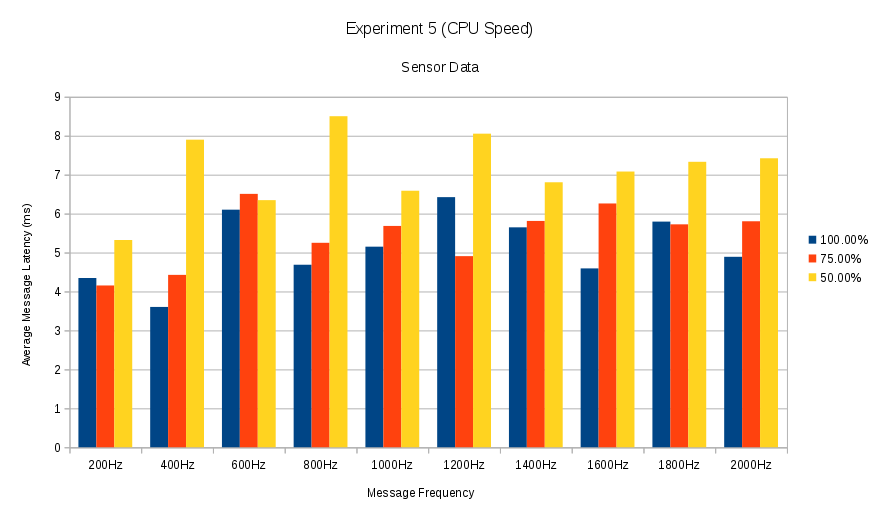
\includegraphics[width=\textwidth]{images/experiment5/sensor_data_all_freqs.png}
\caption{Experiment 5 - Sensor Data, All Frequencies}
\label{exp5-sensor-means-all-freq}
\end{figure}

\begin{figure}[H]
\centering
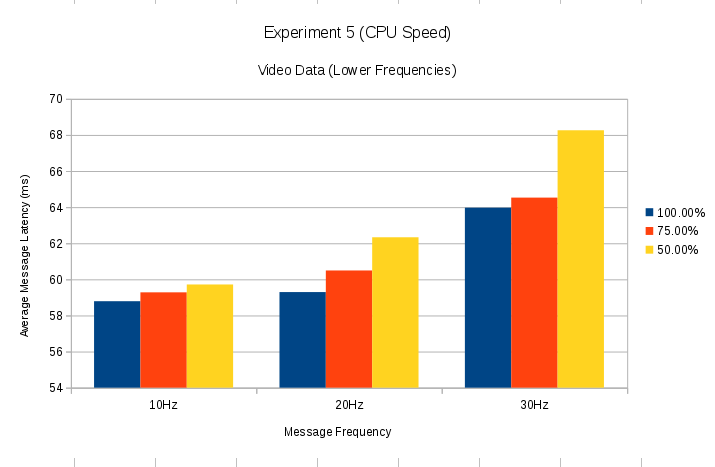
\includegraphics[width=\textwidth]{images/experiment5/video_data_low_freqs.png}
\caption{Experiment 5 - Video Data, Low Frequencies}
\label{exp5-video-means-low-freq}
\end{figure}

\begin{figure}[H]
\centering
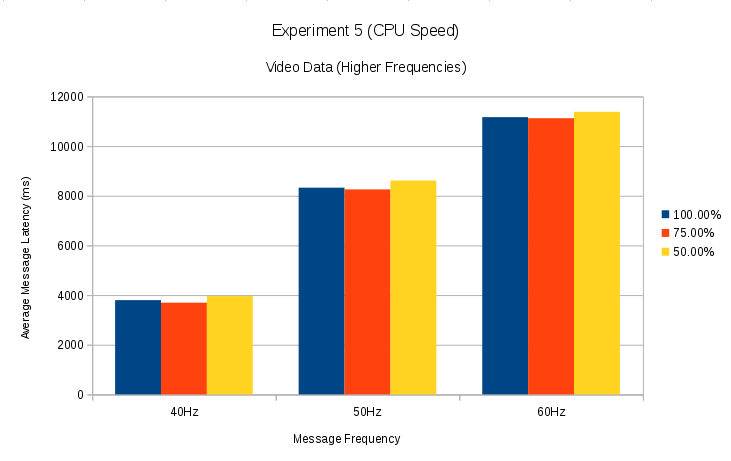
\includegraphics[width=\textwidth]{images/experiment5/video_data_higher_freqs.png}
\caption{Experiment 5 - Video Data, High Frequencies}
\label{exp5-video-means-high-freq}
\end{figure}

\end{document}
